\documentclass[12pt]{article}
\usepackage[T1]{fontenc}
\usepackage{graphicx}
\usepackage{float}
\usepackage[polish]{babel}
\usepackage{amsmath}

\setlength{\textheight}{21cm}

\title{{\bf Zadanie nr 1 - Generacja sygnału\\ i szumu}\linebreak
Cyfrowe Przetwarzanie Sygnałów}
\author{Jakub Wąchała, 216914 \and Radosław Grela, 216769}
\date{24.03.2020}

\begin{document}
\clearpage\maketitle
\thispagestyle{empty}
\newpage
\setcounter{page}{1}
\section{Cel zadania}
\label{cel}
Celem zadania jest oswojenie się z podstawowymi rodzajami sygnałów, dokładnie z wybranymi ich cechami poprzez napisanie programu, który pozwoli na:
\begin{enumerate}
\item Generowanie sygnałów i szumu o ustalonych przez nas parametrach:
\begin{itemize}
\item szum o rozkładzie jednostajnym
\item szum gaussowski
\item sygnał sinusoidalny
\item sygnał sinusoidalny wyprostowany jednopołówkowo
\item sygnał sinusoidalny wyprostowany dwupołówkowo
\item sygnał prostokątny
\item sygnał prostokątny symetryczny
\item sygnał trójkątny
\item skok jednostkowy
\item impuls jednostkowy
\item szum impulsowy
\end{itemize}
\item Wykonanie na nich operacji takich jak:
\begin{itemize}
\item dodawanie
\item odejmowanie
\item mnożenie
\item dzielenie
\end{itemize}
\item Możliwość przedstawienia sygnałów w postaci graficznej tj. wykres i histogram
\item Zapis i odczyt z pliku sygnałów wymienionych powyżej
\end{enumerate}

\section{Wstep teoretyczny}
Program jest aplikacją okienkową, napisany w języku Python (środowisko PyCharm). Wykresy i histogramy generowane są za pomocą biblioteki  \texttt{matplotlib.pyplot}, natomiast 
do stworzenia GUI wykorzystaliśmy bibliotekę  \texttt{tkinter}. Po uruchomieniu programu użytkownikowi ukazuje się menu:
\begin{figure}[H]
\centering
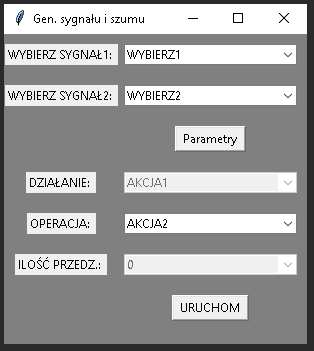
\includegraphics[scale=0.8]{menu11.png}
\caption{Menu główne}
\end{figure}
Z listy należy wybrać sygnał/sygnały (istnieje możliwość wyboru sygnału z pliku), którym jesteśmy zainteresowani. 
\begin{figure}[H]
\centering
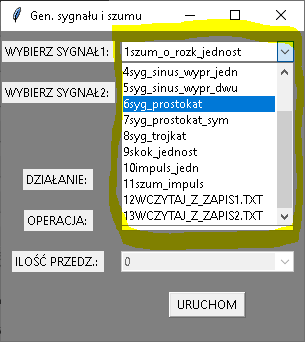
\includegraphics[scale=0.8]{menu12.png}
\caption{Wybór sygnału}
\end{figure}
Następnie należy wcisnąć przycisk "{Parametry}" { }po czym pojawi się okno, aby uzupełnić szczegóły sygnału (paramerty nieprzydatne wypełniamy zerami):
\begin{figure}[H]
\centering
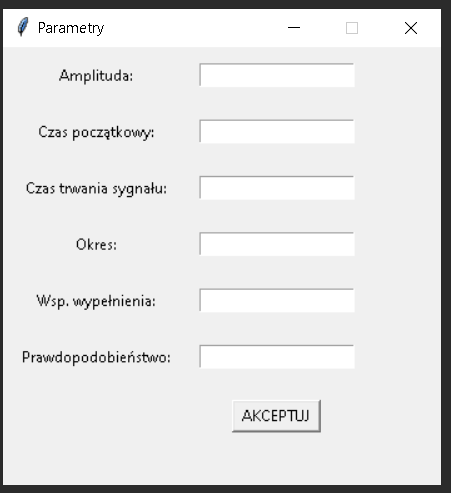
\includegraphics[scale=0.65]{menu22.png}
\caption{Menu wyboru parametrów tworzenia sygnału/szumu}
\end{figure}
W przypadku nie wypełnienia wszystki pól zostanie wyświetlony komunikat o błędzie:
\begin{figure}[H]
\centering
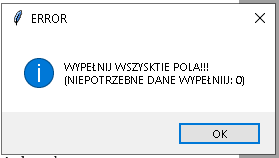
\includegraphics[scale=0.9]{menu33.png}
\caption{Komunikat o błędzie przy wypełnianiu parametrów}
\end{figure}
Kolejny krok to wybór akcji jaką chcemy wykonać na wybranym sygnale:
\begin{itemize}
\item możliwe operacje po wybraniu jednego sygnału:
\begin{figure}[H]
\centering
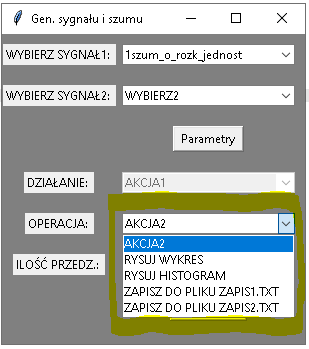
\includegraphics[scale=0.9]{menu44.png}
\caption{Możliwe operacje dla jednego sygnału}
\end{figure}
\item Po wybraniu dwóch sygnałów (oprócz możliwości jakie zapewnia wybór tylko jednego) mamy możliwość (a nawet konieczność) wyboru działania na sygnałach:
\begin{figure}[H]
\centering
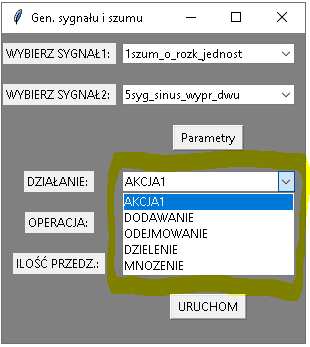
\includegraphics[scale=0.9]{menu55.png}
\caption{Dodatkowe działania dla dwóch sygnałów}
\end{figure}
\item W przypadku wyboru operacji "{RYSUJ HISTOGRAM}"{ }odblokowywane jest pole "ILOŚĆ PRZEDZIAŁÓW"{ }gdzie wybieramy (0,5,10,15) jako ich ilość w histogramie.
\begin{figure}[H]
\centering
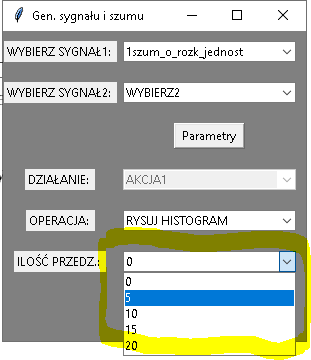
\includegraphics[scale=0.9]{menu66.png}
\caption{Wybór ilości przedziałów histogramu}
\end{figure}
\end{itemize}
Po kliknięciu przycisku "{URUCHOM}"{ }otrzymamy wynik wybranej przez nas operacji wraz z okienkową informacją o: 
\begin{itemize}
\item wartość średnia
\item wartość średnia bezwzględna
\item wartość skuteczna
\item wariancja
\item moc średnia
\end{itemize}
wybranego sygnału:

\begin{figure}[H]
\centering
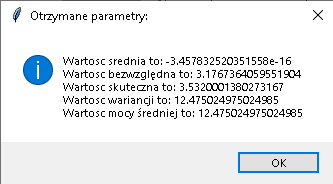
\includegraphics[scale=1.0]{menu77.png}
\caption{Przykład otrzymanych parametrów}
\end{figure}

\section{Eksperymenty i wyniki}
Eksperymenty jakie przeprowadzimy w tym punkcie to przedstwienie czterech pojedynczych sygnałów, a także dodatkowo cztery sygnały, które będą wynikami operacji kolejno: dodawania, odejmowania, mnożenia i dzielenia. 
\subsection{Sygnał sinusoidalny}
Celem eksperymentu jest wygenerowanie sygnału sinusoidalnego.
\label{syg1}
\subsubsection{Założenia\( ^{[\ref{zad1}]}\)}
\label{wzor1}
Funkcja opisująca sygnał:
\begin{equation} 
x(t) = Asin(\frac{2\pi}{T}(t - t_1))
\end{equation}
Użyte parametry:
\begin{itemize}
\item amplituda: 15
\item okres: 5
\item czas początkowy: 0
\item czas trwania: 20
\end{itemize}
\subsubsection{Rezultat}
\begin{figure}[H]
\centering
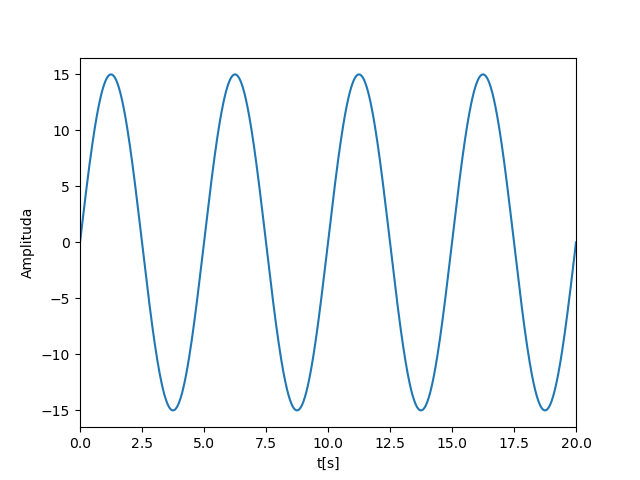
\includegraphics[scale=0.8]{sygSinusWykres.png}
\caption{Wykres sygnału sinusoidalnego}
\end{figure}
\begin{figure}[H]
\centering
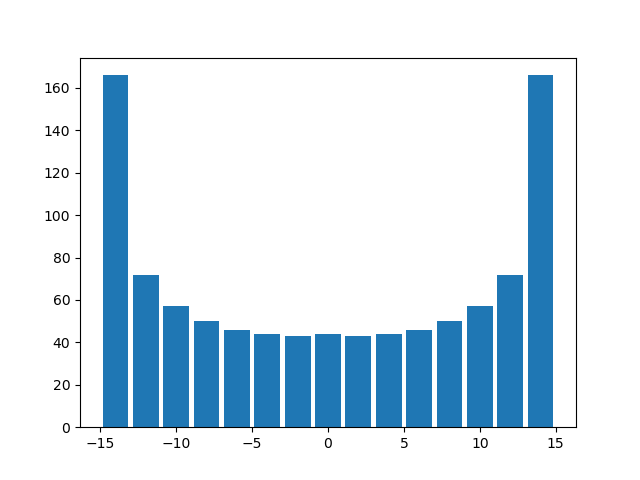
\includegraphics[scale=0.8]{sygSinusHist.png}
\caption{Histogram sygnału sinusoidalnego}
\end{figure}
\begin{figure}[H]
\centering
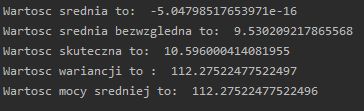
\includegraphics[scale=0.8]{sygSinusParam.png}
\caption{Otrzymane wartości dla sygnału sinusoidalnego}
\end{figure}

\subsection{Sygnał prostokątny}
Celem eksperymentu jest wygenerowanie sygnału prostokątnego.
\label{syg2}
\subsubsection{Założenia\( ^{[\ref{zad1}]}\)}
\label{wzor2}
Funkcja opisująca sygnał:
\begin{equation}
x(t) =
\begin{cases}
A\text{ }dla\text{ }t\in <k{T}+t_1,k_w{T}+k{T}+t_1)\\
0\text{ } dla\text{ } t\in <k_wT-kT+t_1,T+kT+t_1)\\
\end{cases}
dla\text{ } k\in C
\end{equation}
Użyte parametry:
\begin{itemize}
\item amplituda: 15
\item okres: 5
\item czas początkowy: 0
\item czas trwania: 20
\end{itemize}
\subsubsection{Rezultat}
\begin{figure}[H]
\centering
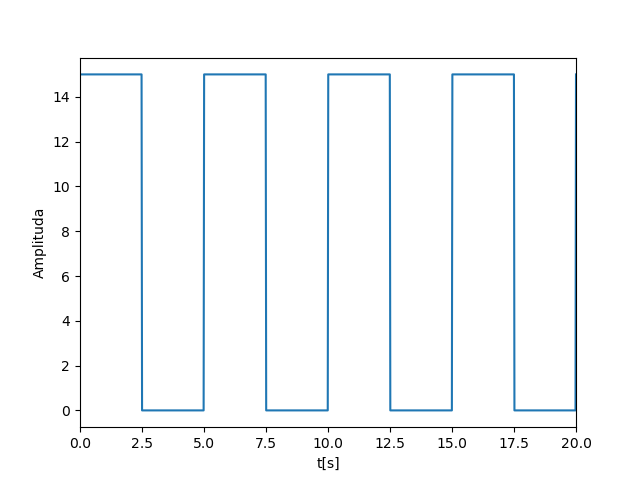
\includegraphics[scale=0.8]{sygProstWykres.png}
\caption{Wykres sygnału prostokątnego}
\end{figure}
\begin{figure}[H]
\centering
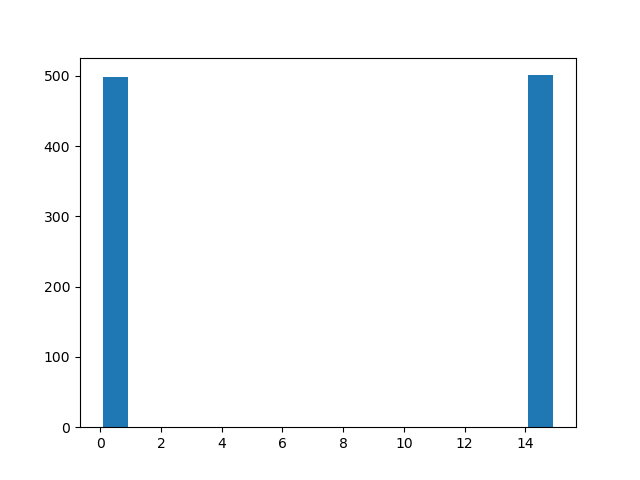
\includegraphics[scale=0.8]{sygProstHist.png}
\caption{Histogram sygnału prostokątnego}
\end{figure}
\begin{figure}[H]
\centering
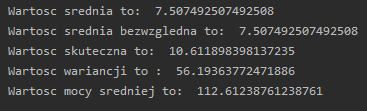
\includegraphics[scale=0.8]{sygProstParam.png}
\caption{Otrzymane wartości dla sygnału prostokątnego}
\end{figure}

\subsection{Sygnał trójkątny}
Celem eksperymentu jest wygenerowanie sygnału trójkątnego.
\label{syg3}
\subsubsection{Założenia\( ^{[\ref{zad1}]}\)}
\label{wzor3}
Funkcja opisująca sygnał:
\begin{equation}
x(t) =
\begin{cases}
\frac{A}{k_wT}(t-kT-t_1) \text{ }dla\text{ }t\in <kT+t_1,k_w{T}+k{T}+t_1)\\
\frac{-A}{T(1-k_w)}(t-kT-t_1)+\frac{A}{1-k_w} \text{ }dla\text{ }t\in <k_w{T}+t_1+kT, T+kT+t_1)\\
\end{cases}
dla\text{ } k\in C
\end{equation}
Użyte parametry:
\begin{itemize}
\item amplituda: 15
\item okres: 5
\item czas początkowy: 0
\item czas trwania: 20
\end{itemize}
\subsubsection{Rezultat}
\begin{figure}[H]
\centering
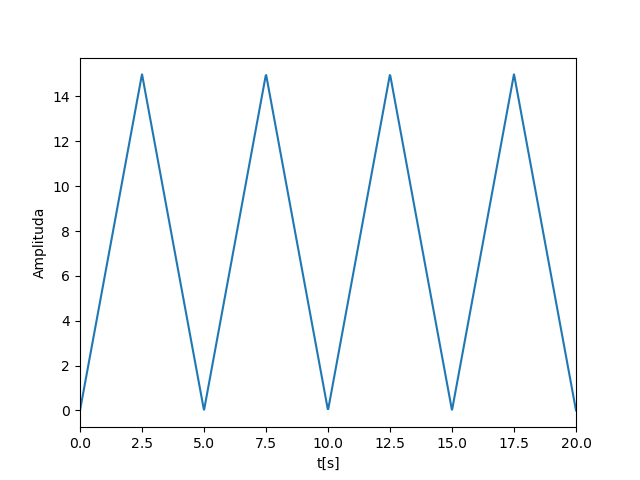
\includegraphics[scale=0.8]{sygTrojkatWykres.png}
\caption{Wykres sygnału trójkątnego}
\end{figure}
\begin{figure}[H]
\centering
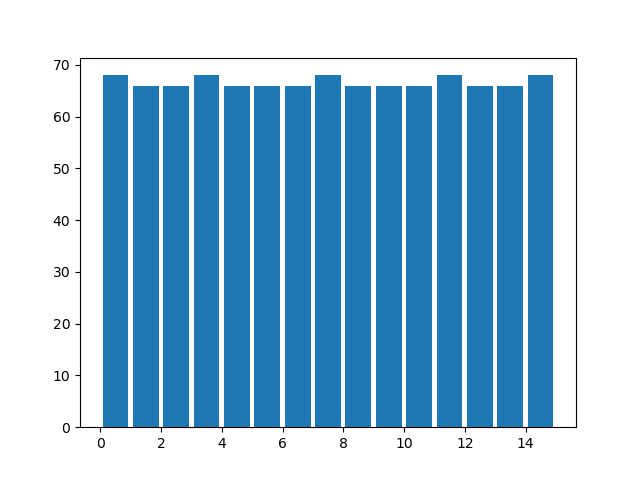
\includegraphics[scale=0.8]{sygTrojkatHist.png}
\caption{Histogram sygnału trójkątnego}
\end{figure}
\begin{figure}[H]
\centering
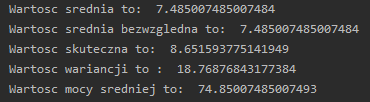
\includegraphics[scale=0.8]{sygTrojkatParam.png}
\caption{Otrzymane wartości dla sygnału trójkątnego}
\end{figure}


\subsection{Szum impulsowy}
Celem eksperymentu jest wygenerowanie szumu impulsowego.
\label{syg4}
\subsubsection{Założenia\( ^{[\ref{zad1}]}\)}
Jest to sygnał dyskretny, którego amplituda przyjmuje dwie wartości, wartość 0 oraz
wartość A różną od zera.
\begin{itemize}
\item  Wystąpienie A uzależnione jest od ustalonego od nas prawdopodobieństwa wystąpienia wartości A
\end{itemize}
Użyte parametry:
\begin{itemize}
\item amplituda: 15
\item czas początkowy: 0
\item czas trwania: 20
\item prawdopodobieństwo wystąpienia wartości A: 70
\end{itemize}
\subsubsection{Rezultat}
\begin{figure}[H]
\centering
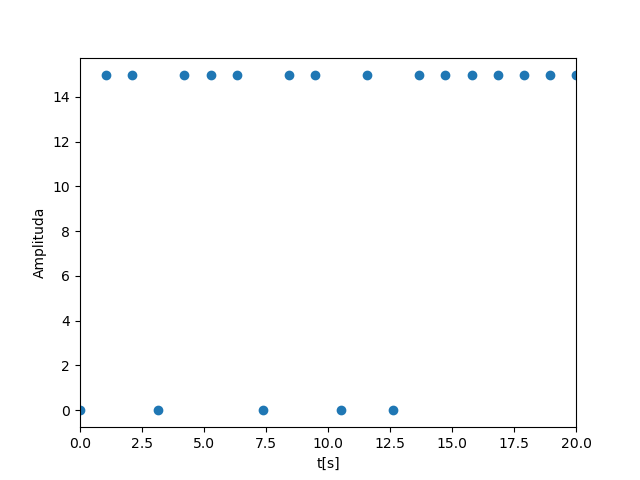
\includegraphics[scale=0.8]{szumImpulsWykres.png}
\caption{Wykres szumu impulsowego}
\end{figure}
\begin{figure}[H]
\centering
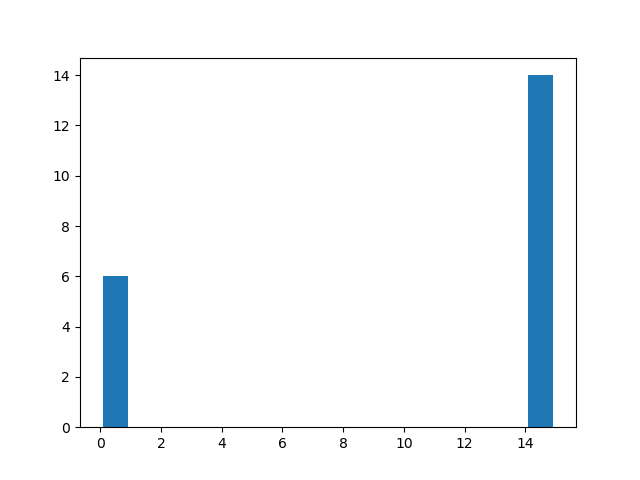
\includegraphics[scale=0.8]{szumImpulsHist.png}
\caption{Histogram szumu impulsowego}
\end{figure}
\begin{figure}[H]
\centering
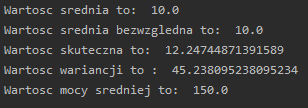
\includegraphics[scale=0.8]{szumImpulsParam.png}
\caption{Otrzymane wartości dla szumu impulsowego}
\end{figure}


\subsection{Dodawanie sygnałów \ref{syg1} (sinusoidalny), \ref{syg2} (prostokątny)}
\label{syg5}
Celem tego eksperymentu jest wygenerowanie sygnału, który jest rezultatem dodawania sygnału  \textbf{\ref{syg1}} oraz  \textbf{\ref{syg2}}.
\subsubsection{Założenia}
Sygnał powstaje w wyniku dodawania sygnałów, które powstały według wzorów:  \textbf{\ref{wzor1}} oraz  \textbf{\ref{wzor2}}.
\subsubsection{Rezultat}
\begin{figure}[H]
\centering
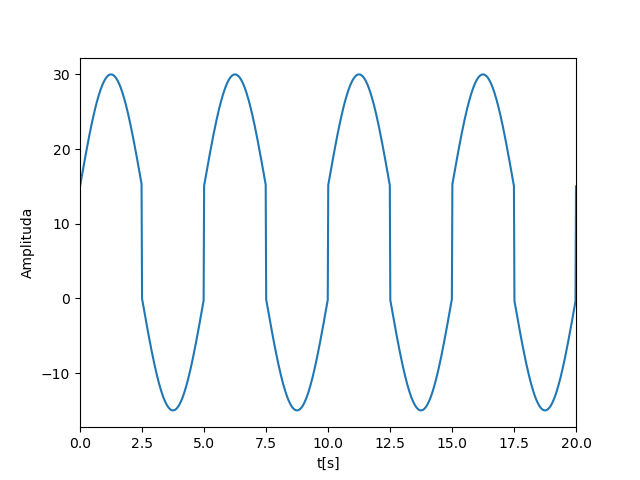
\includegraphics[scale=0.8]{dodawanieSinusProstWykres.png}
\caption{Wykres dla powstałego sygnału}
\end{figure}
\begin{figure}[H]
\centering
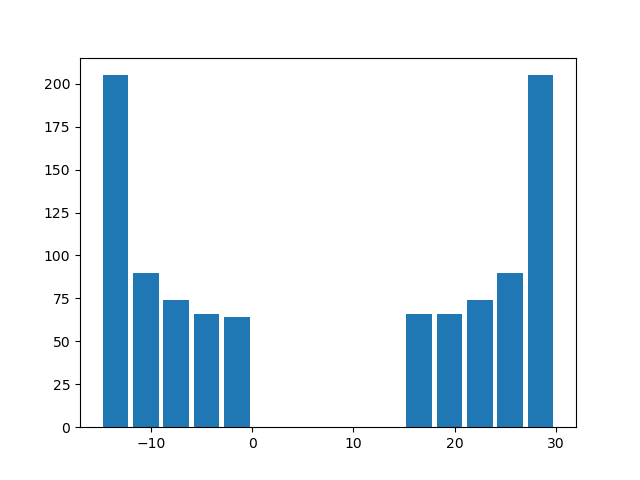
\includegraphics[scale=0.8]{dodawanieSinusProstHist.png}
\caption{Histogram dla powstałego sygnału}
\end{figure}
\begin{figure}[H]
\centering
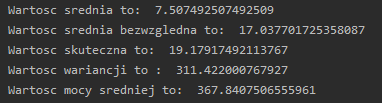
\includegraphics[scale=0.8]{dodawanieSinusProstParam.png}
\caption{Otrzymane wartości dla powstałego sygnału}
\end{figure}


\subsection{Odejmowanie sygnałów \ref{syg2} (prostokątny), \ref{syg3} (trójkątny)}
\label{syg6}
Celem tego eksperymentu jest wygenerowanie sygnału, który jest rezultatem odejmowania sygnału  \textbf{\ref{syg2}} oraz  \textbf{\ref{syg3}}.
\subsubsection{Założenia}
Sygnał powstaje w wyniku odejmowania sygnałów, które powstały według wzorów:  \textbf{\ref{wzor2}} oraz  \textbf{\ref{wzor3}}.
\subsubsection{Rezultat}
\begin{figure}[H]
\centering
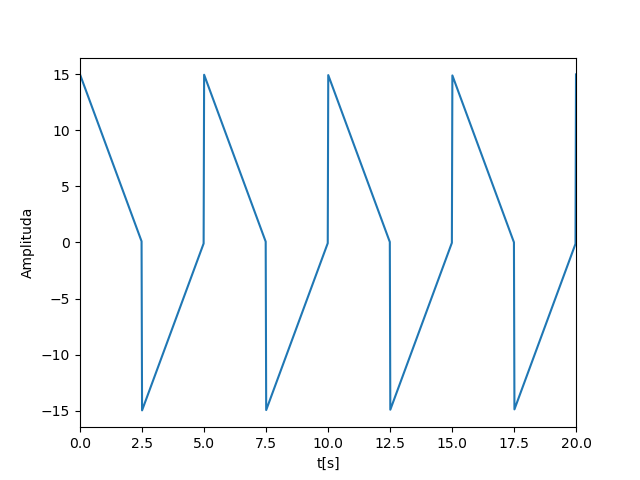
\includegraphics[scale=0.8]{odejmowanieProstTrojkWykres.png}
\caption{Wykres dla powstałego sygnału}
\end{figure}
\begin{figure}[H]
\centering
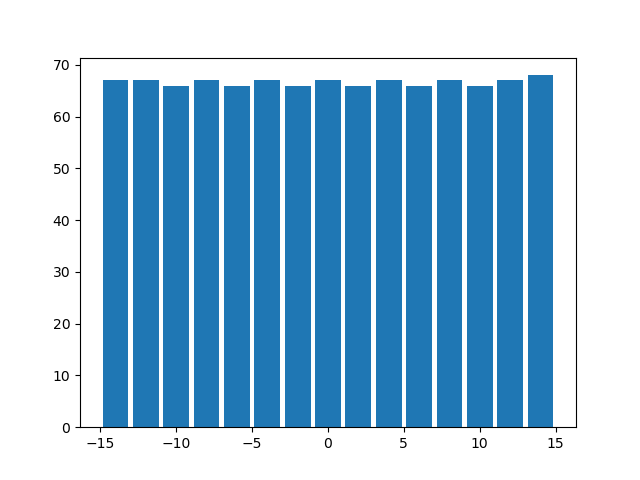
\includegraphics[scale=0.8]{odejmowanieProstTrojkHist.png}
\caption{Histogram dla powstałego sygnału}
\end{figure}
\begin{figure}[H]
\centering
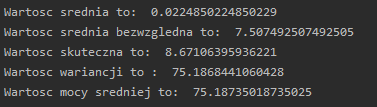
\includegraphics[scale=0.8]{odejmowanieProstTrojkParam.png}
\caption{Otrzymane wartości dla powstałego sygnału}
\end{figure}

\subsection{Mnożenie sygnałów \ref{syg1} (sinusoidalny), \ref{syg3} (trójkątny)}
\label{syg7}
Celem tego eksperymentu jest wygenerowanie sygnału, który jest rezultatem mnożenia sygnału  \textbf{\ref{syg1}} oraz  \textbf{\ref{syg3}}.
\subsubsection{Założenia}
Sygnał powstaje w wyniku mnożenia sygnałów, które powstały według wzorów:  \textbf{\ref{wzor1}} oraz  \textbf{\ref{wzor3}}.
\subsubsection{Rezultat}
\begin{figure}[H]
\centering
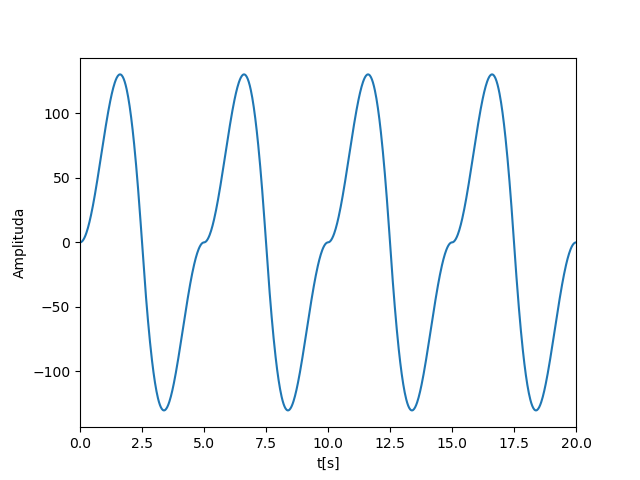
\includegraphics[scale=0.8]{mnozenieSinusTrojkatWykres.png}
\caption{Wykres dla powstałego sygnału}
\end{figure}
\begin{figure}[H]
\centering
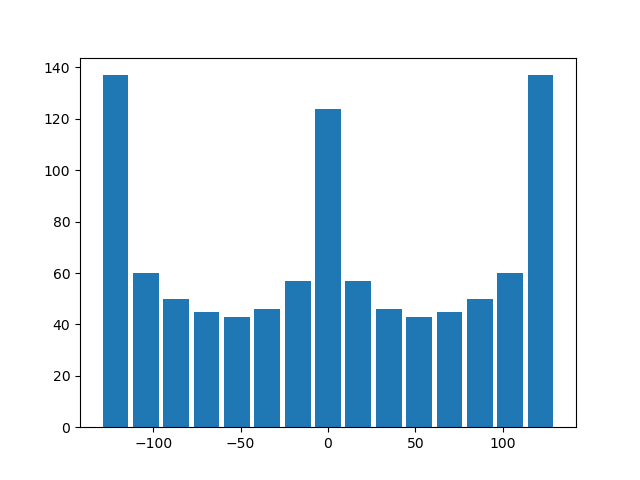
\includegraphics[scale=0.8]{mnozenieSinusTrojkatHist.png}
\caption{Histogram dla powstałego sygnału}
\end{figure}
\begin{figure}[H]
\centering
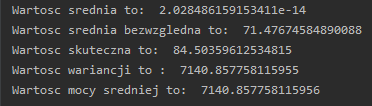
\includegraphics[scale=0.8]{mnozenieSinusTrojkatParam.png}
\caption{Otrzymane wartości dla powstałego sygnału}
\end{figure}

\subsection{Dzielenie sygnałów \ref{syg1} (sinusoidalny), \ref{syg2} (prostokątny)}
\label{syg8}
Celem tego eksperymentu jest wygenerowanie sygnału, który jest rezultatem dzielenia sygnału  \textbf{\ref{syg1}} oraz  \textbf{\ref{syg2}}.
\subsubsection{Założenia}
Sygnał powstaje w wyniku dzielenia sygnałów, które powstały według wzorów:  \textbf{\ref{wzor1}} oraz  \textbf{\ref{wzor2}}.
\subsubsection{Rezultat}
\begin{figure}[H]
\centering
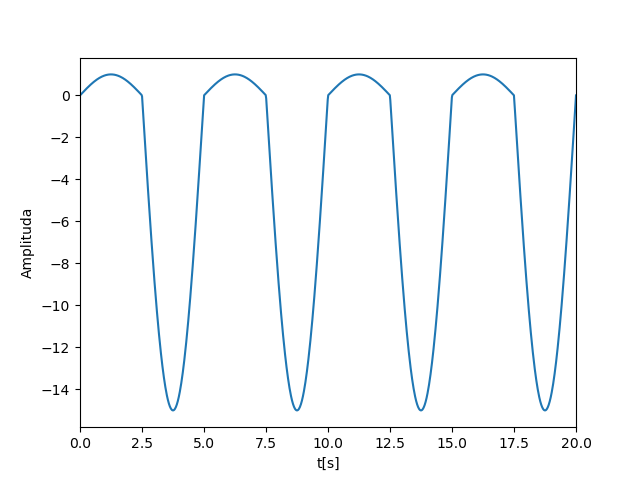
\includegraphics[scale=0.8]{dzielenieSinusProstWykres.png}
\caption{Wykres dla powstałego sygnału}
\end{figure}
\begin{figure}[H]
\centering
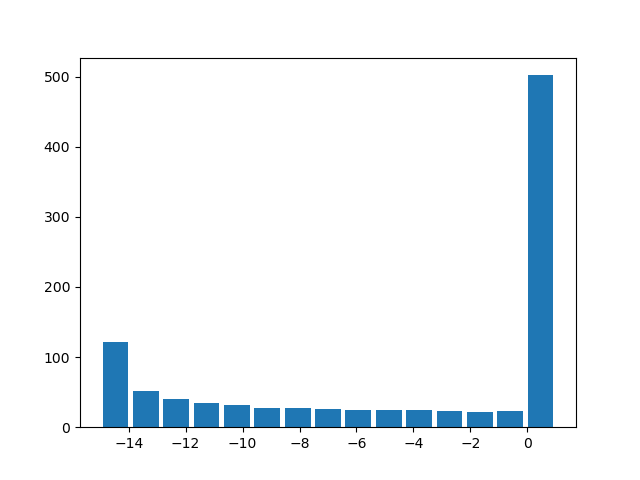
\includegraphics[scale=0.8]{dzielenieSinusProstHist.png}
\caption{Histogram dla powstałego sygnału}
\end{figure}
\begin{figure}[H]
\centering
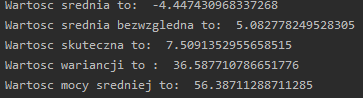
\includegraphics[scale=0.8]{dzielenieSinusProstParam.png}
\caption{Otrzymane wartości dla powstałego sygnału}
\end{figure}

\section{Wnioski}
Podczas tworzenia programu dołożyliśmy wszelkich starań, aby nasz program spełniał wszystkie wymagania pozwalające na poprawne zrealizowanie zadania.
Zadanie to pozwoliło nam wzbogacić naszą wiedzę i umiejętności w zakresie sygnałów, szumów, impulsów oraz operacji na nich. A także dało nam nowe spojrzenie na szerokie możliwości jakich dostarcza nam język Python w kwestii tworzenia wszelkiej maści wykresów i histogramów.

\begin{thebibliography}{0}
\bibitem{bib1}
\label{zad1}
\textit{Zadanie 1 - Generacja sygnału i szumu} Cyfrowe Przetwarzanie Sygnału WIKAMP FTIMS\newline
\end{thebibliography}

\end{document}